\chapter{Four Wave Mixing}
\label{ch:FWM}

The average power of a single frequency of light calculated from Eq.~\ref{eq:average_power} will be constant over time. If two frequencies are present, their interference will cause the average power to vary sinusoidally over time. Since $\gamma\neq0$ implies that the refractive index depends on power, the simultaneous presence of two frequencies of light in a nonlinear medium implies that the phase will be sinusoidally modulated. This effect generates new frequency components and is referred to as "Four Wave Mixing" (FWM).




\section{Electrical phase modulation}
To understand FWM, first consider a continuous wave laser signal launched into a commercially available phase modulator being driven by an sinusoidal electrical signal from a function generator. See Fig.~\ref{fig:PM} for a visualization and \href{https://youtu.be/j8It3to54AQ}{this video} for an experimental demonstration. The signal at the output is given by
\begin{align}
    \label{eq:phase_modulator}
    \E_{out}&=\E_{in}\exp\left(i\Phi\cos(\omega_dT), \right)
\end{align}
where $\Phi$ is the maximum phase shift imparted by the modulator and $\omega_d$ is the modulation frequency. See \href{https://www.desmos.com/calculator/vcreo1gs2q}{this interactive graph} for an illustration of the impact of this modulation on the real part of $\E_{out}$. Using the so-called "Jacobi-Anger Expansion"~\cite{NIST_JA_expansion}, the cosine function inside the complex exponential in Eq.~\ref{eq:phase_modulator} can be written as
\begin{align}
\label{eq:JA}
    \exp\left(i\Phi\cos(\omega_dT)\right) &= \sum_{n=-\infty}^{\infty}i^n J_n(\Phi) \exp\left(in\omega_dT\right),
\end{align}
where $J_n(\Phi)$ is the $n^{th}$ order Bessel function of the 1st kind. In short, Eq.~\ref{eq:JA} shows that sinusoidal phase modulation gives rise to new discrete frequency components spaced $\omega_d$ apart and whose relative powers depend on the modulation amplitude, $\Phi$. Note also that applying Eq.~\ref{eq:chirp_definition} to Eq.~\ref{eq:phase_modulator} shows that the sinusoidal modulation changes the instantaneous frequency over time by $\Phi\omega_d\sin(\omega_dT)$, further suggesting that phase modulation changes the color of the incident light.

\begin{figure}
    \centering
    \includegraphics[width=1\linewidth]{figures/PhaseModulator.png}
    \caption{Illustration of the impact of electrical sinusoidal phase modulation of a continuous wave optical signal. Before entering the modulator, only a single laser frequency is present. After the modulator, the alternating advancement and delay of the optical phase in the time domain is equivalent to introducing new frequency components according to Eq.~\ref{eq:JA}.}
    \label{fig:PM}
\end{figure}

\section{Nonlinearity based phase modulation}
\label{sec:sidebands}
The following approach to modelling FWM is inspired by the one originally presented in~\cite{Boskovic_Original_Kerr_Effect}. Consider Eq.~\ref{eq:SPM_applied} and assume that the field, $\A(0,T)$ can be written as the sum of two continuous wave signals with average powers $P_a$ and $P_b$ and a frequency spacing of $\Delta\omega$ according to
\begin{align}
    \label{eq:FWM_input}
    \A(0,T)&= \sqrt{P_a}e^{-i\frac{\Delta\omega}{2}T}+\sqrt{P_b}e^{i\frac{\Delta\omega}{2}T}.
\end{align}
When the signal consists of two pulses with finite durations, the continuous wave assumption is an approximation, which is valid when $\omega_d$ is larger than the bandwidths of the pulses. The field at the end of the nonlinear medium is
\begin{align}
    \A(L,T) &= \A(0,T)\exp\left(i\gamma L [P_a+P_b+2\sqrt{P_aP_b}\cos(\omega_dT)] \right) \\ \nonumber
    &= \A(0,T)\exp\left(i\gamma L [P_a+P_b]\right)\exp\left(i2\gamma L\sqrt{P_aP_b}\cos(\omega_dT) \right)\\ \nonumber
    \A(L,T)Q^{-1}&= \A(0,T)\exp\left(i2\gamma L\sqrt{P_aP_b}\cos(\omega_dT) \right)\\ \nonumber
    \A(L,T)Q^{-1}&= \A(0,T)\exp\left(i\phi_{NL}\cos(\omega_dT) \right),
\end{align}
where the time-independent factor $Q=\exp(i\gamma L [P_a+P_b])$ is temporarily moved to the left hand side of the equality for convenience. Applying Eq.~\ref{eq:JA} yields
\begin{align}
    \A(L,T)Q^{-1}&= \A(0,T)\sum_{n=-\infty}^{\infty}i^nJ_n(\phi_{NL})e^{in\omega_dT} \\ \nonumber
    &=\left(\sqrt{P_a}e^{-i\frac{\Delta\omega}{2}T}+\sqrt{P_b}e^{i\frac{\Delta\omega}{2}T}\right)\sum_{n=-\infty}^{\infty}i^nJ_n(\phi_{NL})e^{in\omega_dT} \\ \nonumber
    &=\sqrt{P_a}\sum_{m=-\infty}^{\infty}i^mJ_m(\phi_{NL})e^{i\left(m-\frac{1}{2}\right)\omega_dT}+...\\ \nonumber & \quad\quad\quad\quad\quad\sqrt{P_b}\sum_{k=-\infty}^{\infty}i^kJ_k(\phi_{NL})e^{i\left(k+\frac{1}{2}\right)\omega_dT}.
\end{align}
Note that the infinite sum initially indexed by $n$ is split into two infinite sums indexed by $m$ and $k$ because the two complex exponentials in $\A(0,T)$ cause the frequency corresponding to $m=1$ in the first sum to be different from the one corresponding to $k=1$ in the second sum. To re-combine the two sums, use $m=k+1$ and obtain
\begin{align}
\label{eq:re_index}
    \A(L,T)Q^{-1}&=\sqrt{P_a}\sum_{k=-\infty}^{\infty}i^{k+1}J_{k+1}(\phi_{NL})e^{i\left(k+\frac{1}{2}\right)\omega_dT}+...\\ \nonumber & \quad\quad\quad\quad\quad\sqrt{P_b}\sum_{k=-\infty}^{\infty}i^kJ_k(\phi_{NL})e^{i\left(k+\frac{1}{2}\right)\omega_dT} \\ \nonumber
    &= \sum_{n=-\infty}^{\infty} i^n\left[i\sqrt{P_a}J_{n+1}\left(\phi_{NL}\right)+\sqrt{P_b}J_n\left(\phi_{NL}\right)\right]e^{i\omega_d\left(n+\frac{1}{2}\right)T}.
\end{align}
Finally, moving $Q$ to the right hand side of Eq.~\ref{eq:re_index} yields
\begin{align}
\label{eq:FWM_general}
    \A(L,T)&=\sum_{n=-\infty}^{\infty} i^n\left[i\sqrt{P_a}J_{n+1}\left(2\gamma L\sqrt{P_aP_b}\right)+\sqrt{P_b}J_n\left(2\gamma L\sqrt{P_aP_b}\right)\right]e^{i\omega_d\left(n+\frac{1}{2}\right)T+i\gamma L[P_a+P_b]}.
\end{align}
In Eq.~\ref{eq:FWM_general}, the frequency component for which $n=-1$ will be at $-\omega_d/2$, while the one for which $n=0$ will be at $+\omega_d/2$, corresponding to the original two frequencies in Eq.~\ref{eq:FWM_input}. The average power of the $n^{th}$ order sideband is
\begin{align}
\label{eq:sideband_power}
    |\A_n(L,T)|^2 &= P_aJ^2_{n+1}\left(2\gamma L \sqrt{P_aP_b}\right)+P_bJ^2_{n}\left(2\gamma L \sqrt{P_aP_b}\right).
\end{align}
See Fig.~\ref{fig:FWM} a) and b) for a numerical simulation of the sideband powers for different values of $2\gamma L \sqrt{P_aP_b}$. See Fig.~\ref{fig:FWM} c) for a comparison of the numerically calculated sideband powers and the ones predicted by Eq.~\ref{eq:sideband_power}. Assuming that $P_a\ll P_b$ and $2\gamma L\sqrt{P_aP_b}<\sqrt{1+n}$ with $n>0$ yields
\begin{align}
\label{eq:sideband_approx}
    |\A_n(L,T)|^2 &\approx P_b\frac{(\gamma^2 L^2P_aP_b)^{n}}{n!^2},
\end{align}
since
\begin{align}
\label{eq:Bessel_approx}
    J_n(x)&\approx \frac{1}{n!}\left(\frac{x}{2}\right)^n
\end{align}
for small arguments in the Bessel function. See Fig.~\ref{fig:FWM} d) for an illustration of the scaling behavior predicted by Eq.~\ref{eq:sideband_approx}. The fact that the power of higher order sidebands is more sensitive to changes in input power than lower order ones is useful for various all-optical signal processing techniques~\cite{my_thesis,BenoitPhD,YangLuPhD}. See \href{https://youtu.be/0SXPvO89jto}{this tutorial video} for a different approach to modelling FWM that takes dispersion into account. See \href{https://youtu.be/gsa9hrCbnqI}{this video} for an experimental demonstration of FWM. 
\begin{figure}
    \centering
    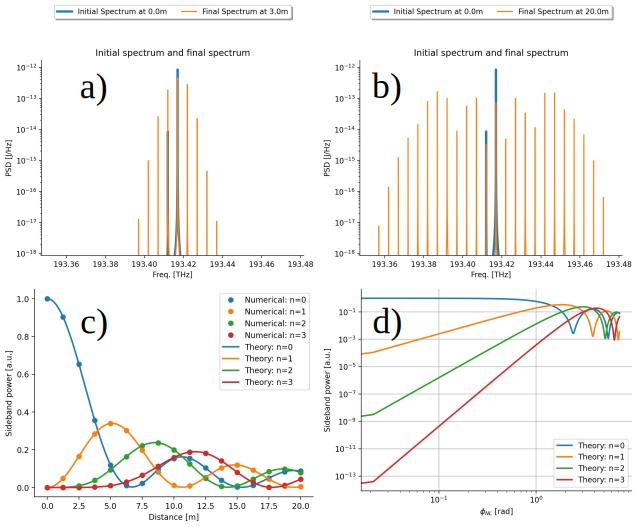
\includegraphics[width=1.0\linewidth]{figures/FWM_combined.png}
    \caption{a) Numerically calculated initial and final spectrum when two frequencies with $P_b=100P_a$ spaced 5~GHz apart  propagate through a medium where $\phi_{NL}=2\gamma L\sqrt{P_aP_b}=1.08$~rad. Note the transfer of power from the most intense frequency into neighbouring sidebands and the rapid decrease in power for increasing sideband orders as predicted by Eq.~\ref{eq:sideband_approx}. b) Same as a) but for $\phi_{NL}=2\gamma L\sqrt{P_aP_b}=7.2$~rad. c) Comparison of sideband power normalized to $P_b$ according to numerical simulations and Eq.~\ref{eq:sideband_power}. d) Similar to c) but plotted on a double-log scale versus $\phi_{NL}$ to demonstrate the scaling behavior predicted by Eq.~\ref{eq:sideband_approx}. Figures generated using \href{https://colab.research.google.com/drive/1l054EDg-50aK5GORN_md4_-tlFy4jwC5?usp=sharing}{this interactive notebook}, which the reader is encouraged to experiment with.   }
    \label{fig:FWM}
\end{figure} 

\section{Cross Phase Modulation (XPM)}
\label{Sec:XPM}
In Chapter~\ref{ch:SPM}, it was shown that the phase of a single-frequency optical field in a nonlinear medium increases linearly with the average power of that field. When two frequencies are present, the phase of one frequency component as a function of its own average power and the average power of the other can be calculated from Eq.~\ref{eq:FWM_general}. Choosing the $n=0$ component yields
\begin{align}
    \phi_0 &= \frac{\omega_d}{2}T+\gamma L [P_a+P_b]+\theta_0,
\end{align}
where
\begin{align}
\label{eq:theta}
    \theta_0 &= arg\left( i\sqrt{P_a}J_{1}\left(2\gamma L\sqrt{P_aP_b}\right)+\sqrt{P_b}J_0\left(2\gamma L\sqrt{P_aP_b}\right) \right) \\ \nonumber
    &= \arctan\left(\frac{\sqrt{P_a}J_{1}\left(2\gamma L\sqrt{P_aP_b}\right)}{\sqrt{P_b}J_0\left(2\gamma L\sqrt{P_aP_b}\right) } \right).
\end{align}
Using Eq~\ref{eq:Bessel_approx} allows Eq.~\ref{eq:theta} to be written as
\begin{align}
    \theta_0 &\approx\arctan\left(\frac{\sqrt{P_a}\gamma L\sqrt{P_aP_b}}{\sqrt{P_b} } \right) \\ \nonumber
    &\approx\arctan\left(\gamma LP_a\right) \\ \nonumber
    &\approx \gamma LP_a.
\end{align}
Thus, the phase of the $n=0$ frequency component is
\begin{align}
    \label{eq:XPM}
    \phi_0 &\approx \frac{\omega_d}{2}T+\gamma L [P_a+P_b]+\gamma LP_a \\ \nonumber
    &=\frac{\omega_d}{2}T+\gamma L [2P_a+P_b].
\end{align}
Note that $n=0$ is the frequency at $+\omega_d/2$, which initially had the average power $P_b$. Therefore, the term in Eq.~\ref{eq:XPM} containing $P_b$ corresponds to the impact of SPM, while the term containing $P_a$ corresponds to so-called "Cross Phase Modulation" (XPM). Interestingly, Eq.~\ref{eq:XPM} shows that XPM is "twice as strong" as SPM as demonstrated numerically in Fig.~\ref{fig:XPM}. See \href{https://youtu.be/aDXd13zLPC4}{this video tutorial} for an alternative derivation starting from Maxwell's Equations of the impact of XPM. See \href{https://www.desmos.com/calculator/vstlwgtlyb}{this interactive graph} for an illustration of the relative impact of SPM and XPM on two waves with different frequencies.

\begin{figure}
    \centering
    \includegraphics[width=0.8\linewidth]{figures/XPM_combined.png}
    \caption{Illustration of the disparate impacts of SPM and XPM on the phase of an optical signal. a) Time domain representation of a low power CW signal overlapped with two identical, high power Gaussian pulses that only differ by their carrier frequencies. The carrier frequency of the pulse on the left is 10~GHz below the carrier frequency of the CW light. b) After simulating the propagation through a nonlinear medium, the CW light obtains approximately twice the phase shift from XPM as from SPM as predicted by Eq.~\ref{eq:XPM}. The ratio of $0.0360/0.0187\approx 1.925\neq2$ is attributed to the approximations involved in Eq.~\ref{eq:XPM} and to the finite time resolution of the simulation. Figures generated using \href{https://colab.research.google.com/drive/1aIRradfOZGN7JYUhbtYJdVzJwAZoYoUe?usp=sharing}{this interactive notebook}, which the reader is encouraged to experiment with.}
    \label{fig:XPM}
\end{figure}






\section{Phase matching}
\label{sec:Phase_matching}
The derivation presented in Section~\ref{sec:sidebands} assumes negligible dispersion, which is the case for a small $\omega_d$ value and a carrier frequency close to the zero dispersion frequency explained in Subsection~\ref{subsec:ZDF}. The impact of dispersion on FWM is explained in \href{https://youtu.be/0SXPvO89jto}{this video tutorial}. It turns out that FWM is weak for positive values of $\betag_2$ and is most significant when
\begin{align}
\label{eq:phase_matching}
0&=\betag_2\omega_d^2+\gamma(P_a+P_b)    \\ \nonumber
\betag_2&=-\gamma(P_a+P_b)/\omega_d^2<0,    
\end{align}
assuming that $\omega_d$ is small enough for $\betag_2$ to be the only relevant term in Eq.~\ref{eq:beta_approx}. The reason is that FWM as a process involves the \emph{coherent} transfer of power from one set of electromagnetic waves into oscillating changes in the refractive index of the nonlinear medium and then into another set of electromagnetic frequencies. In short, the nonlinearity ensures that the incident electromagnetic waves will cause the tiny dipoles constituting the medium to oscillate at new temporal frequencies. If the corresponding spatial frequency of one of these temporal oscillations in the dipoles is the same as the spatial frequency of another electromagnetic wave, its power will increase with distance via constructive interference as explained in \href{https://youtu.be/bha8SzWzRc4}{this video tutorial}. The requirement in Eq.~\ref{eq:phase_matching} arises because the difference in spatial frequencies of the incident waves and the new wave should be small and because the increase in the refractive index due to the power of the initial fields makes the spatial frequencies larger than they normally would be. Thus, a negative values of $\betag_2$ is needed to compensate. This effect, where the spatial frequencies caused by the regular refractive index of the medium balance changes in the spatial frequencies due field power via nonlinearity, is referred to as "phase matching". The phase matching condition in Eq.~\ref{eq:phase_matching} is relevant for the special case of FWM and similar expressions can be derived for other nonlinear effects beyond the scope of this primer, such as \href{https://www.youtube.com/watch?v=UpuN0dS23Nw}{Second-Harmonic generation} , \href{https://youtu.be/bha8SzWzRc4}{Third-Harmonic generation} and \href{https://www.creol.ucf.edu/mir/wp-content/uploads/sites/7/2023/07/L22_-Stimulated-Brillouin-scattering.pdf}{Stimulated Brillouin Scattering}.  

\subsection{Modulation Instability}
As a consequence of FWM, a signal with a carrier frequency where $\betag_2<0$ for a particular nonlinear medium will get noisier as it propagates forward. The reason is that the interference between the carrier and tiny, ubiquitous fluctuations in the electromagnetic field will cause FWM to transfer optical power away from the carrier and into adjacent frequencies as explained \href{https://prefetch.eu/know/concept/modulational-instability/}{here} and illustrated in Fig.~\ref{fig:MI}. The process of particular noise frequencies being preferentially amplified due to phase matching is referred to as "Modulation Instability" (MI). See \href{https://youtu.be/VtaoPd0Fwj8}{this video tutorial} for further details on MI. 

\begin{figure}
    \centering
    \includegraphics[width=0.75\linewidth]{figures/MI_combined.png}
    \caption{a) Initial and final time domain power of a signal consisting of a Gaussian pulse and random noise with an amplitude 1.000 times smaller than that of the Gaussian propagated through 100m of a nonlinear medium with $\betag_2<0$. b) Same as a) but showing the spectrum. c-d) Same as a-b) but for a distance of 200m. e-f) Same as a-b) but for a distance of 300m. g) full temporal evolution for 500m. h) Same as g) but for the spectrum. Figures generated using \href{https://colab.research.google.com/drive/1p2aQZ4zPPAIMplVxvlezdmpQt_j-rsY7?usp=sharing}{this interactive notebook}, which the reader is encouraged to experiment with.}
    \label{fig:MI}
\end{figure}



